\section{Zielsetzung}
\label{sec:Zielsetzung}
Ziel diese Versuches ist die Anwendung der Tomographie als bildgebendes Verfahren, um die Zusammensetzung verschiedener Würfel zu bestimmen.
Hierbei wird Gammastrahlung verwendet.

\section{Theorie}
\label{sec:Theorie}
In diesem Abschnitt wird die Theorie des Versuchs erklärt, indem zuerst allgemein erklärt wird, was genau die Tomographie ist und wie der Absorptionskoeffizient bestimmt wird.
Anschließend wird die Gammastrahlung betrachtet mit einem besonderem Augenmerk auf dem Zerfall von Caesium und den verschiedenen Wechselwirkungen von Gammastrahlung mit Materie . 

\subsection{Tomographie}
\label{subsec:Tomographie}
Die Tomographie ist ein bildgebendes Verfahren, welches hauptsächlich zur Untersuchung von räumlichen Strukturen benutzt wird,
indem mehrere Querschnittsbilder bzw. Projektionen erstellt werden.
Es beruht auf dem Prinzip der Absorption. Dabei wird ein Objekt mit Gammastrahlung bestrahlt und es wird vor und nach der Transmission die
Intensität gemessen. Abhängig vom Material wird die Strahlung unterschiedlich stark absorbiert. Die Materialen besitzen somit verschiedene
Absorptionskoeffizienten $\mu_i$.
Nach der Transmission durch das Objekt kann die Intensität nach Lambert-Beer zu
\begin{equation*}
    I = I_0 \text{e}^{-\sum_i \mu_i d_i}
\end{equation*}
bestimmt werden, wobei $I_0$ die Anfangsintensität, $\mu_i$ der Absorptionskoeffizient und $d_i$ die Wegstrecke sind.
Diese Formel kann umgestellt werden zu
\begin{equation}
    \sum_i \mu_i d_i = \text{ln}\biggl(\frac{I_0}{I_j}\biggr),
    \label{eqn:mu}
\end{equation}
was die Möglichkeit schafft, ein Gleichungssystem zu bilden, mit dessen Hilfe die Zusammensetzung verschiedener Materialien in einem nicht
einsehbaren Körper bestimmt werden kann.
Dafür wird die Messung verschiedener Intensitäten $I_j$ und eine geschickte Auswahl von Strahlwegen benötigt.

\subsection{Gammastrahlung und der Caesium Zerfall}
\label{subsec:GammaCaesium}
In diesem Versuch wird eine Gammaquelle benutzt, weswegen im Folgenden die Gammastrahlung betrachtet wird. Wenn Gammastrahlung auf Matrie trifft,
treten verschiedene Wechselwirkungen auf, welche die Absorption und somit die Abschwächung der Intensität beeinflussen. 

\subsubsection{Phototeffekt}
\label{subsubsec:Phototeffekt}
Der Phototeffekt dominiert bei niedrigen Energien bis ungefähr $\qty{100}{\kilo\electronvolt}$.
Dabei trifft ein Photon auf ein kernnahes Schalenelektron eines Atoms und gibt dabei seine ganze Energie ab.
Ist die Photonenergie höher als die Bindungsenergie des Elektrons, so wird dieses aus der Schale ausgelöst.
Das Photoelektron besitzt anschließend die überschüssige Energie des Photons. Diese kinetische Energie entspricht der Differenz aus Photonenergie
und der Austrittsarbeit.

\subsubsection{Comptoneffekt}
\label{subsubsec:Comptoneffekt}
Bei dem Comptoneffekt trifft das Photon auf ein kernentferntes Elektron, wobei diese in einem inelastischen Stoß wechselwirken.
Dabei gibt das Photon nur ein Teil seiner Energie ab und erfährt eine Richtungsänderung und eine Änderung seiner Wellenlänge
\begin{equation}
    \Delta \lambda = \frac{h}{m c} \biggl(1 - \text{cos}(\theta)\biggr).
\end{equation}
Das Elektron erfährt eine Impulsänderung.
Der Comptoneffekt dominiert bei Energien zwischen $\qty{0.1}{\mega\electronvolt}$ und $\qty{1}{\mega\electronvolt}$.

\subsubsection{Paarbildung}
\label{subsubsec:Paarbildung}
Die Paarbildung tritt erst bei höheren Energien auf, um genau zu sein ab der doppelten Ruheenergie des Elektrons (ca. $\qty{1.02}{\mega\eV}$).
Das Photon wird unter Erzeugung eines Elektrons und Positrons ausgelöscht.
Es wird Energie an den Atomkern abgegeben, aufgrund des Impulserhaltungsatzes.
Die Paarerzeugung kann jedoch in diesem Versuch vernachlässigt werden, weil die Energie der Gammastrahlung in diesem Versuch nicht hoch genug ist.

\subsubsection{Caesium Zerfall}
\label{subsubsec:Caesium}
Caesium $\ce{^{137}Cs}$ ist ein Alkalimetall und zerfällt mit einer Wahrscheinlichkeit von $\qty{94.6}{\percent}$ über einen $\beta^-$-Zerfall
in ein metastabiles $\ce{^{137}Ba}$.
Durch Aussendung eines Gammaquants mit einer Energie von $\qty{0.662}{\mega\eV}$ zerfällt es weiter in den stabilen Zustand von $\ce{^{137}Ba}$.
Mit einer Wahrscheinlichkeit von $\qty{5.4}{\percent}$ zerfällt $\ce{^{137}Cs}$ direkt in den stabilen Zustand von $\ce{^{137}Ba}$.
Der Caesium-Zerfall ist in \autoref{fig:Zerfall} dargestellt.
\begin{figure}[H]
    \centering
    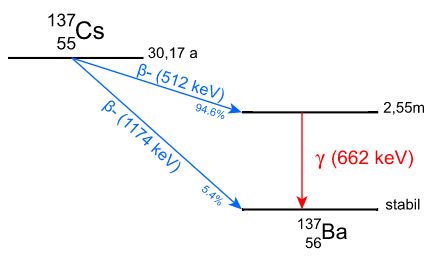
\includegraphics[scale=0.7]{Abbildungen/Caesiumzerfall.png}
    \caption{Schematische Darstellung des Caesium-Zerfalls.\cite{Gammaspektrum}}
    \label{fig:Gammaspektrum}
\end{figure}



\subsection{Messung der Absorptionskoeffizienten}
\label{subsec:Absorptionskoeffizient}
Um ein dreidimensionales Bild zu erzeugen, werden verschiedene Projektionen aus unterschiedlichen Richtungen benötigt.
Im Folgenden wird mit der Matrixschreibweise gearbeitet, wobei
\autoref{eqn:mu} zu
\begin{equation}
    A \vec{\mu} = \vec{I}
    \label{eqn:muMatrix}
\end{equation}
umgeschrieben wird. Dabei ist $\vec{\mu}$ der bestimmende Vektor der Absorptionskoeffizienten, $A$ ist die Matrix, die Informationen über die
Wegstrecken enthält und $\vec{I}$ ist der Vektor der gemessenen Intensitäten gemäß der rechten Seite von \autoref{eqn:mu}.\\
Der Durchführung vorwegnehmend wird ein Würfel bestehend aus $3 \times 3 \times 3$ Elementarwürfeln und umgeben von einer Aluminiumhülle benutzt.
Es wird aus Zeitgründen nur eine Schicht untersucht. Daraus folgt, dass neun Absorptionskoeffizienten bestimmt werden.
Somit hat der Vektor für die Absorptionskoeffizienten $n = 9$ Dimensionen und die Matrix $A$ besitzt die 
Dimension $m \times n$. Dabei ist $m$ die Dimension des Vektors $\vec{I}$, also die Anzahl der durchgeführten Messungen.
Um das lineare Gleichungssystem mit einem klassischen Ansatz lösen zu können, sind mindestens $n$ unterschiedliche Projektionen zu wählen,
wobei sichergestellt werden muss, dass die resultierende Matrix $A$ nicht singulär ist. 
Es empfiehlt sich jedoch, zu Gunsten einer besseren Statistik mehr Messungen bzw. Projektionen durchzuführen.
Dabei zeigt \autoref{fig:Ausrichtung} die zwölf ausgewählten Projektionen zur Untersuchung einer Schicht des Würfels.

\begin{figure}[H]
    \centering
    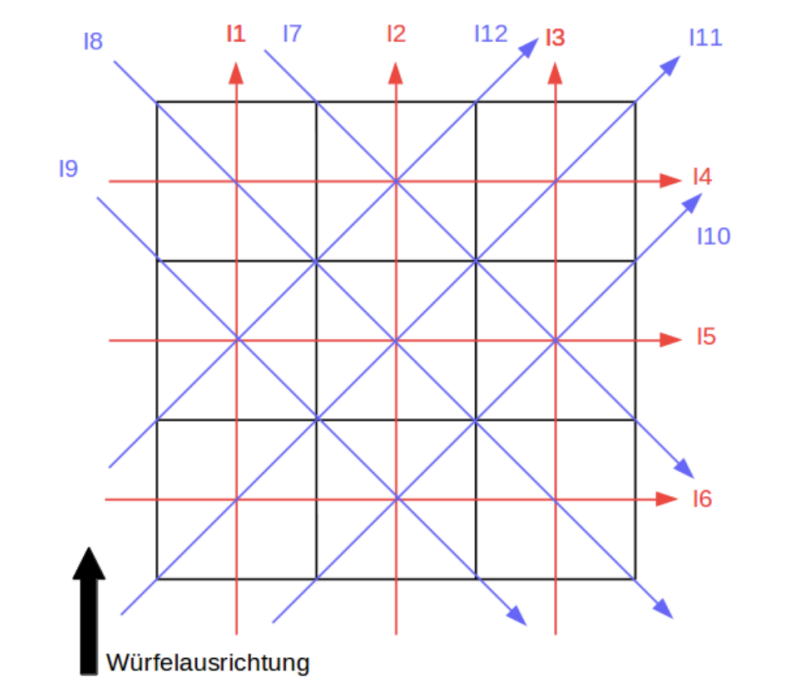
\includegraphics[scale=0.7]{Abbildungen/Ausrichtung.png}
    \caption{Darstellung der zwölf gewählten Projektionen für die mittlere 3 × 3 Schicht eines zu untersuchenden Würfels.\cite{V14}}
    \label{fig:Ausrichtung}
\end{figure}

Mit der Methode der kleinsten Quadrate kann \autoref{eqn:muMatrix} umgeschrieben werden zu
\begin{equation}
    W \,A \,\vec{\mu} = W \,\vec{I},
\end{equation}
wobei $W$ die Gewichtungsmatrix
\begin{equation}
    W = V[I]^{-1}
\end{equation}
ist, welche über die Inverse Varianz der Intensität definiert ist. Daraus ergibt sich für $\vec{\mu}$ die Relation
\begin{equation}
    \vec{\mu} = \biggl(A^T\, W \,A\biggr)^{-1} \biggl(A^T \,W \,\vec{I}\biggr)
    \label{eqn:mu_gleichung}
\end{equation}
und die Unsicherheit ergibt sich aufgrund des Poissonfehler zu
\begin{equation}
    V[\mu] = \biggl(A^T\, W \,A\biggr)^{-1}.
    \label{eqn:Unsicherheit}
\end{equation}



